% Section 1 - Middleware in robotics
% Roberto Masocco <roberto.masocco@uniroma2.it>
% March 13, 2022

% ### Middleware in robotics ###
\section{Middleware in robotics}
\graphicspath{{figs/section1/}}

% --- What is middleware? ---
\begin{frame}{What is middleware?}
\begin{figure}
    \centering
    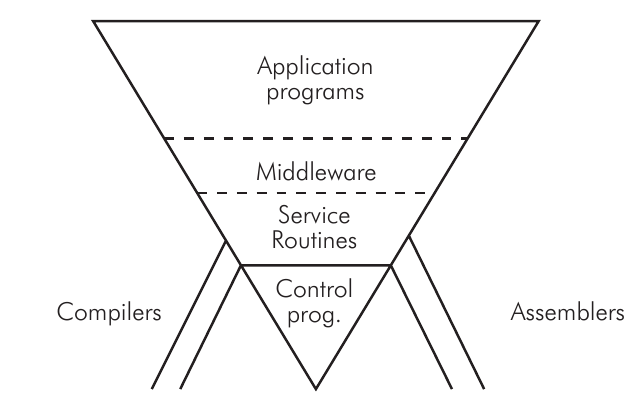
\includegraphics[width=.85\textwidth]{softwarePyramid.png}
    \caption{Software organization in a generic computer system}
    \label{fig:swpyramid}
\end{figure}
\end{frame}
\begin{frame}{What is middleware?}
\begin{block}{Definition of middleware}
    \justifying
    The term \textbf{middleware} identifies a kind of software that offers common services and functionalities to applications in addition to what an operating system usually does.
\end{block}
\justifying
Middlewares are usually implemented as \textbg{libraries} that application programmers can use via appropriate \textbg{APIs}.
\end{frame}

% --- Middleware in robotics ---
\begin{frame}{Middleware in robotics}
\justifying
Classic problems arising when developing software for autonomous systems:
\begin{itemize}
    \item definition of tasks;
    \item hardware integration;
    \item software organization and maintenance;
    \item communication and data exchange (involves both hardware and software!);
    \item debugging and testing.
\end{itemize}
\begin{block}{}
    \centering
    Middlewares can offer services to tackle and solve each one!
\end{block}
\end{frame}

% --- Data Distribution Service ---
\begin{frame}{Data Distribution Service}
\begin{block}{Definition of DDS}
    A DDS is a \textbf{publish-subscribe middleware} that handles communications between \textbf{real-time} systems and software over the network.
\end{block}
DDS implementations follow an open standard that defines:
\begin{itemize}
    \item serialization and deserialization of data packets;
    \item automatic discovery of \textbg{DDS participants} (over \textbg{multicast-IP/UDP}) and transmission of data (over \textbg{unicast-IP/UDP});
    \item \textbg{security protocols} and cryptographic operations;
    \item enforcing of \textbg{Quality of Service} policies to organize transmissions (specifying things like \textbg{queue sizes}, \textbg{best-effort} or \textbg{reliable} transmissions...).
\end{itemize}
DDSs are currently used in automotive, aerospace, military...
\end{frame}
\begin{frame}{Data Distribution Service}
\begin{figure}
    \centering
    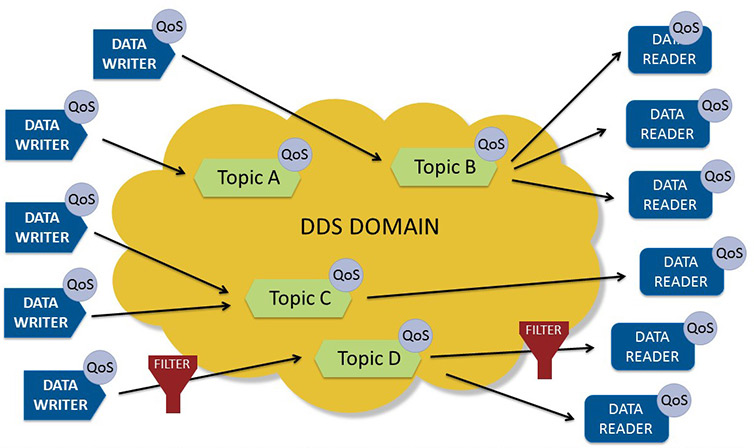
\includegraphics[width=.85\textwidth]{ddsDomain.jpg}
    \caption{Scheme of a DDS-based network}
    \label{fig:ddsdomain}
\end{figure}
\end{frame}
\begin{frame}{Data Distribution Service}
DDS participants can either \textbg{publish to} or \textbg{subscribe to} a \textbg{topic}.
\begin{block}{Definition of DDS topic}
    A DDS topic is uniquely identified by three things:
    \begin{itemize}
        \item a \textbf{name}, i.e. a human-readable character string;
        \item an \textbf{interface}, i.e. a custom packet format that specifies what data is carried over it (e.g. strings, numbers, arrays...);
        \item a \textbf{QoS policy} that specifies how transmissions should be performed.
    \end{itemize}
\end{block}
\begin{block}{}
    \centering
    Changing even only one of the above results in a completely different topic!
\end{block}
\end{frame}
